\documentclass[conference]{IEEEtran}
\IEEEoverridecommandlockouts
\usepackage[nocompress]{cite}
\usepackage{amsmath,amssymb,amsfonts}
\usepackage{graphicx}
\usepackage{textcomp}
\usepackage{booktabs}
\usepackage{url}
\usepackage{multirow}

\begin{document}

\title{Confidently Wrong: Silent Failures of Classical and Learned Feature Matching for GPS-Denied UAV Localization}

\author{
\IEEEauthorblockN{Kana Am\'ed\'ee}
\IEEEauthorblockA{Independent Researcher \\
Bujumbura, Burundi \\
kanaamedee00@gmail.com \\
ORCID 0009-0009-9620-6399 \\
Code: github.com/kanaamedee11/confidently-wrong-skygaze}
}

\maketitle

\par\noindent{\small\bfseries\itshape Abstract. }{\small\bfseries A GPS-denied UAV can fall back on matching its camera view against a stored georeferenced reference image. Matchers are usually compared by accuracy alone, but a navigation system also needs to know when a match is wrong. We present SkyGaze, an open pipeline that runs SIFT, ORB and SuperPoint+SuperGlue behind one interface, and classify every trial as accurate, a detected failure, or a silent failure (a wrong homography returned as a success). Using exact ground truth over 3{,}474 synthetic trials, we sweep in-plane rotation and six further degradations. SuperGlue is the most accurate matcher up to $45^\circ$ of rotation (150 of 150 trials, 0.26\,px median error) but collapses within the next $15^\circ$: from $60^\circ$ upward it is accurate in 3 of 150 trials and returns a wrong homography in 79\%, while SIFT and ORB stay above 97\% accurate from $0^\circ$ to $180^\circ$. Evaluating four rotated copies of the query removes the failure (126 of 126 accurate) at four times the runtime, and the RANSAC inlier count separates correct from wrong results with AUROC 0.999. A smaller check on 32 held-out real UAV-VisLoc frames matched to the real satellite map (96 trials per method) shows the same structure at much lower accuracy: SuperGlue is accurate in 12\% of trials and silently wrong in 61\%, SIFT is accurate in 19\%, and rotation hypotheses raise SuperGlue to 47\%.\par}
\vspace{0.6\baselineskip}
\par\noindent{\small\bfseries\itshape Keywords. }{\small\bfseries visual localization, UAV navigation, GPS-denied navigation, feature matching, SuperGlue, failure analysis, selective prediction\par}

\section{Introduction}

Autonomous UAVs increasingly operate where GPS cannot be trusted: urban canyons that occlude satellites, deliberate jamming, and remote regions with degraded correction signals. When GPS is lost, a UAV usually still has an onboard camera and a stored georeferenced reference image of the area it expects to overfly, such as a satellite tile or an orthophoto. \emph{Visual localization} uses these two to recover position without any satellite signal: the live frame (the \emph{query}) is matched against the reference, and the estimated geometric relation gives the vehicle's location.

The problem is studied under several names, including cross-view geo-localization, terrain-referenced navigation, and GPS-denied visual localization \cite{zheng2020university,zhu2021vigor,goforth2019gps}. A recurring design choice is how the query and reference are matched: with hand-crafted local features such as SIFT \cite{lowe2004distinctive} and ORB \cite{rublee2011orb}, or with a learned matcher such as SuperPoint and SuperGlue \cite{detone2018superpoint,sarlin2020superglue}. Comparisons between them are usually reported as accuracy on a benchmark. For a navigation system, a second question matters at least as much: \emph{when a matcher fails, does the system know?} A matcher that declines to answer is an inconvenience; a matcher that confidently returns a wrong position is a hazard, because the downstream controller has no reason to distrust it.

This paper builds a small, fully reproducible harness to study exactly that, and reports six contributions.
\begin{enumerate}
\item \textbf{A modular pipeline and evaluation harness.} SkyGaze runs SIFT, ORB and SuperPoint+SuperGlue behind one interface with identical geometric verification, so differences are attributable to the matching stage.
\item \textbf{An outcome taxonomy.} Every trial is classified as \emph{accurate}, \emph{detected failure} (no homography), or \emph{silent failure} (a wrong homography returned as a success). Counting any returned homography as success, as is common, hides the third class entirely.
\item \textbf{A controlled study with exact ground truth} over in-plane rotation and six further degradation axes (scale, perspective, noise, blur, occlusion, appearance), with 3{,}474 synthetic trials in total and confidence intervals.
\item \textbf{A sharp failure mode of the learned matcher, and a cheap remedy.} SuperGlue is the most accurate method up to $45^\circ$ of rotation but collapses within the next $15^\circ$, returning wrong homographies. Evaluating four rotated copies of the query and keeping the hypothesis with the most RANSAC inliers removes the failure at four times the cost.
\item \textbf{A confidence-gate analysis.} We show how well the RANSAC inlier count separates correct from silently wrong localizations, as a risk-coverage trade-off \cite{elyaniv2010foundations}.
\item \textbf{A real-data check.} On 32 held-out frames of a real UAV-VisLoc flight matched against its real satellite map, the same three outcomes are measured in metres (Section~\ref{sec:real}).
\end{enumerate}
We are explicit about scope: the controlled study is synthetic, with queries that are transformed crops of the reference, so its absolute numbers do not transfer to real drone imagery. The real-data check uses one flight, one satellite map and 32 frames, so it tests whether the failure structure carries over and does not establish rates for UAV-VisLoc as a whole.

\section{Related Work}

\textbf{Cross-view geo-localization.} University-1652 \cite{zheng2020university} frames drone, satellite and ground views of the same place as a multi-view retrieval problem, and VIGOR \cite{zhu2021vigor} moves beyond one-to-one retrieval toward finer, city-scale localization. Goforth and Lucey \cite{goforth2019gps} address GPS-denied UAV localization directly against pre-existing satellite imagery with learned features. UAV-VisLoc \cite{xu2024uavvisloc} pairs 6{,}742 real drone images with 11 georeferenced satellite maps and per-image ground truth, and is the benchmark we target for real-data evaluation.

\textbf{Local feature matching.} SIFT \cite{lowe2004distinctive} and ORB \cite{rublee2011orb} remain standard baselines because they are fast, interpretable and need no training data; both are followed by geometric verification, typically RANSAC \cite{fischler1981random}. SuperPoint \cite{detone2018superpoint} learns keypoints and descriptors, and SuperGlue \cite{sarlin2020superglue} learns the matching itself with attention over keypoint sets; its outdoor weights are trained on MegaDepth \cite{li2018megadepth}. Detector-free LoFTR \cite{sun2021loftr} and the faster LightGlue \cite{lindenberger2023lightglue} are more recent; we do not evaluate them here (Section~\ref{sec:limits}).

\textbf{Knowing when to abstain.} Selective prediction studies the trade-off between the fraction of inputs a model answers (coverage) and its error on the answered ones (risk) \cite{elyaniv2010foundations}. We apply this view to localization: a geometric-verification score (the RANSAC inlier count) is the confidence signal, and a threshold on it is the gate.

\section{Method}

\subsection{Problem and pipeline}
Given a reference image $R$ and a query $Q$, the goal is a homography $H$ mapping query pixels to reference pixels, from which the vehicle position, taken as the image of the query centre $c_Q$, is $\hat{p}=H c_Q$. Fig.~\ref{fig:pipeline} shows the pipeline. Keypoints are extracted and matched, RANSAC \cite{fischler1981random} (5.0\,px reprojection threshold, shared by all matchers) estimates $H$ and an inlier set, and a confidence gate decides whether to accept the result.

\begin{figure*}[t]
\centering
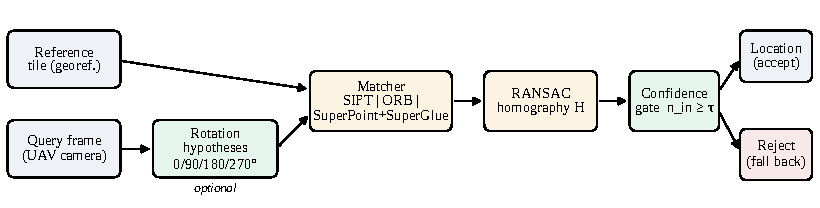
\includegraphics[width=0.96\textwidth]{figures/fig_pipeline_v2.pdf}
\caption{SkyGaze pipeline. The matcher is swappable behind one interface. Two stages are optional additions studied here: rotation hypotheses in front of the matcher, and a confidence gate on the RANSAC inlier count after it.}
\label{fig:pipeline}
\end{figure*}

\subsection{Matchers}
\textbf{SIFT} \cite{lowe2004distinctive}: brute-force L2 matching with Lowe's ratio test at 0.75. \textbf{ORB} \cite{rublee2011orb}: up to 4000 features, Hamming matching with the same ratio test. \textbf{SuperGlue} \cite{sarlin2020superglue}: SuperPoint keypoints (at most 1024, threshold 0.005) matched with the pretrained outdoor weights and a match threshold of 0.2. No matcher is tuned on the benchmark.

\subsection{Rotation hypotheses}
Because the cliff reported in Section~\ref{sec:rot} is a function of in-plane rotation, we add a test-time variant, \emph{SuperGlue + rot.\ hyp.}: the query is rotated by $0^\circ$, $90^\circ$, $180^\circ$ and $270^\circ$, each version is matched against the reference, and the hypothesis with the most RANSAC inliers is kept, with its homography composed with the known rotation. Any residual rotation is at most $45^\circ$, inside the range where plain SuperGlue is reliable. The cost is four forward passes.

\subsection{Outcomes, metrics and the confidence gate}
The localization error is $e=\lVert H c_Q - p^{*}\rVert$, in pixels of the $800\times800$ reference, where $p^{*}$ is the exact ground-truth position. A trial is \emph{accurate} if a homography is returned and $e\le\tau$ with $\tau=10$\,px (1.25\% of the reference width); a \emph{silent failure} if a homography is returned with $e>\tau$; and a \emph{detected failure} if none is returned. We report the accurate rate with 95\% Wilson intervals \cite{wilson1927probable}, and the median error among accurate trials.

The gate accepts a result when its RANSAC inlier count is at least $\tau_n$. Sweeping $\tau_n$ gives a risk-coverage curve: coverage is the fraction of all trials accepted, and risk is the fraction of accepted trials that are wrong. We also report the AUROC with which the inlier count separates accurate from non-accurate trials.

\section{Experimental Protocol}

\textbf{Data.} Three procedurally generated $800\times800$ references (fields, a road network and buildings on textured ground, seeds 0 to 2) provide scenes with known structure and no third-party imagery. A query is a $280\times280$ sub-region at a random offset, warped by a known transform, so the ground-truth homography is exact. To test dependence on texture statistics we repeat the rotation sweep on a second domain: a $2\times2$ mosaic of four photographic ground textures (gravel, grass, brick, rotated gravel) from the scikit-image sample data. Fig.~\ref{fig:data} shows the references and one example query per degradation.

\begin{figure*}[t]
\centering
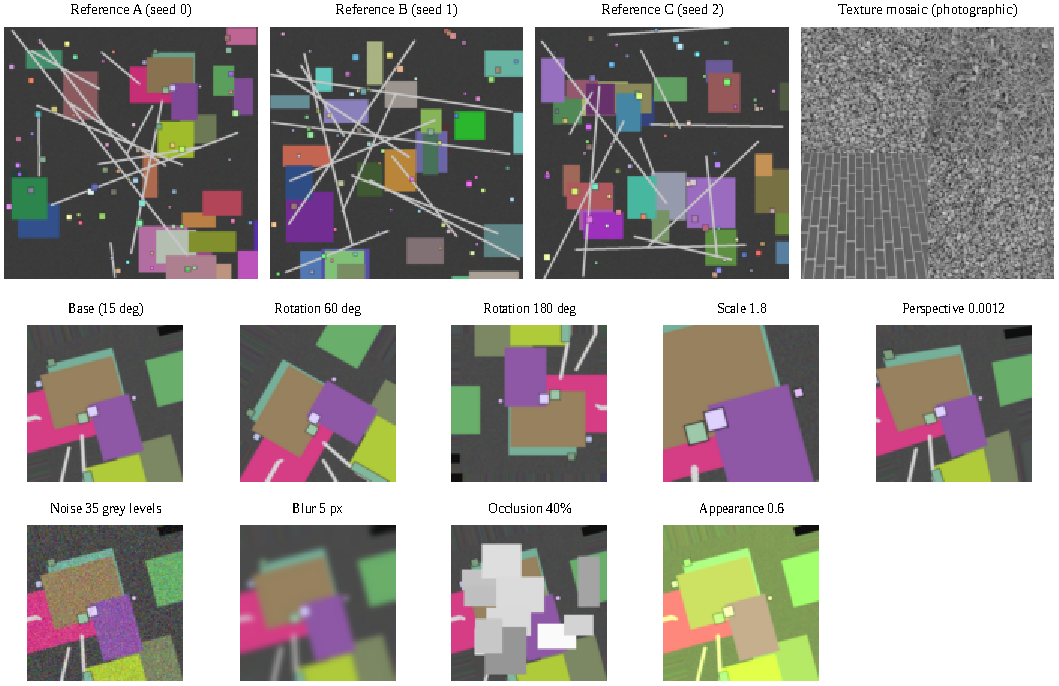
\includegraphics[width=0.86\textwidth]{figures/fig_data_v2.pdf}
\caption{Test imagery. Top: the three generated $800\times800$ reference scenes and the photographic texture mosaic. Below: example $280\times280$ queries cut from Reference A at one location, each showing one degradation at the level named in its title (the base condition is $15^\circ$ rotation, scale 0.9).}
\label{fig:data}
\end{figure*}

\textbf{Degradation axes.} Rotation is swept alone at scale 0.9. The six other axes are swept one at a time around a base condition (rotation $15^\circ$, scale 0.9, brightness $+15$, blur $\sigma=0.8$\,px): scale (query zoom) in $\{0.5, 0.7, 0.9, 1.3, 1.8\}$; a perspective coefficient in $\{0, 2, 4, 8, 12\}\times10^{-4}$ (at the highest value the apparent scale changes by about $\pm17\%$ across the frame edge); additive Gaussian noise $\sigma\in\{0,10,20,35\}$ grey levels; blur $\sigma\in\{0.8,2,3.5,5\}$\,px; occlusion by opaque rectangles covering $\{0,20,40,60\}\%$ of the query; and an appearance gap, a random per-channel gain and global gamma change of strength $\{0,0.2,0.4,0.6\}$.

\textbf{Trial counts.} Rotation: SIFT and ORB 30 trials per angle over 10 angles; SuperGlue 30 per angle over the same angles plus $50^\circ$ and $55^\circ$; the rotation-hypothesis variant 18 per angle over 7 angles. Stress axes: 30 trials per level for SIFT and ORB and 12 for SuperGlue, over 26 levels. Real data: 96 trials per method (32 frames, 3 offsets). Texture domain: 20 trials per cell for SIFT and ORB over 10 angles, 12 for SuperGlue over 7, and 8 for the rotation-hypothesis variant over 4. Every matcher sees the same references and seeds. All runs are on CPU (2 vCPU); SuperGlue uses the public pretrained outdoor weights. Code, trial-level results and the figure scripts are included with the project.

\textbf{Measurement note.} The pipeline's original localization estimate was the mean of the four projected query corners. This equals the projection of the query centre only for similarity transforms; under a perspective component it does not, and would have reported a spurious failure on the perspective axis. All errors here use $H c_Q$.

\section{Results}

\subsection{Rotation: a cliff, not a slope}
\label{sec:rot}
Fig.~\ref{fig:rot} and Table~\ref{tab:rot} show accuracy against in-plane rotation. SIFT (293 of 300 trials accurate, 97.7\%, 95\% CI 95.3 to 98.9) and ORB (300 of 300, 100\%, CI 98.7 to 100) are flat across the full $0^\circ$ to $180^\circ$ range, with median errors of 0.43 and 0.56\,px. SuperGlue is the most accurate method where it works: 150 of 150 trials from $0^\circ$ to $45^\circ$ (CI 97.5 to 100) with a median error of 0.26\,px. It then fails abruptly. A finer sweep shows 97\% accurate at $50^\circ$, 57\% at $55^\circ$, and 10\% at $60^\circ$; from $75^\circ$ to $180^\circ$ it is accurate in none of 120 trials. Over all 150 trials at $60^\circ$ and beyond, SuperGlue returns a homography in 81\% of them but is accurate in only 3 (2\%); 79\% are silent failures and 19\% are detected failures.

\begin{figure*}[t]
\centering
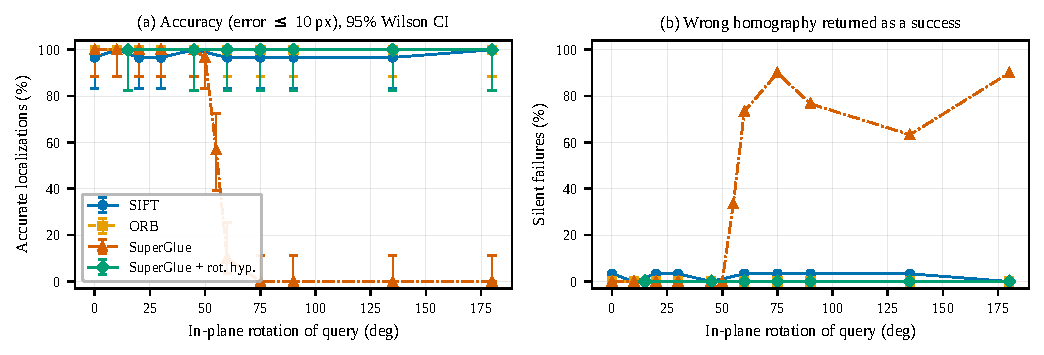
\includegraphics[width=0.98\textwidth]{figures/fig_rotation_v2.pdf}
\caption{Effect of in-plane rotation. (a) Share of trials with a localization error of at most 10\,px, with 95\% Wilson intervals (30 trials per cell for SIFT, ORB and SuperGlue; 18 for the rotation-hypothesis variant). (b) Share of trials in which a wrong homography was returned as a success.}
\label{fig:rot}
\end{figure*}

\begin{table*}[t]
\centering
\caption{Accurate localizations (\%) against in-plane rotation (deg). n/a: not run at that angle. Cells have 30 trials except SuperGlue + rot.\ hyp. (18).}
\label{tab:rot}
\begin{tabular}{@{}l*{10}{r}@{}}
\toprule
Method & 0 & 30 & 45 & 50 & 55 & 60 & 75 & 90 & 135 & 180 \\
\midrule
SIFT & 97 & 97 & 100 & n/a & n/a & 97 & 97 & 97 & 97 & 100 \\
ORB & 100 & 100 & 100 & n/a & n/a & 100 & 100 & 100 & 100 & 100 \\
SuperGlue & 100 & 100 & 100 & 97 & 57 & 10 & 0 & 0 & 0 & 0 \\
SuperGlue + rot.\ hyp. & n/a & n/a & 100 & n/a & n/a & 100 & 100 & 100 & 100 & 100 \\
\bottomrule
\end{tabular}
\end{table*}

Fig.~\ref{fig:qual} shows a typical failure at $75^\circ$: the SuperGlue footprint lands about 1{,}400\,px from the truth, yet the system reports a homography with no warning, while the rotation-hypothesis variant and SIFT recover the correct place. The warning sign is visible in the match statistics: across all SuperGlue trials, accurate results have a median of 58 RANSAC inliers (minimum 6) and wrong results a median of 4 (maximum 10).

\begin{figure*}[t]
\centering
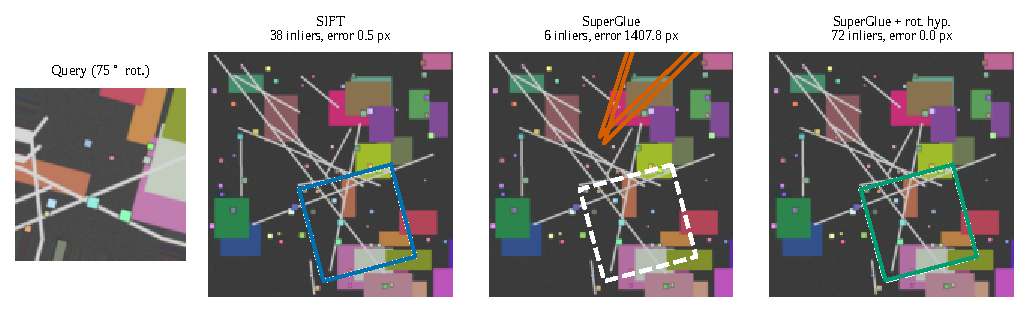
\includegraphics[width=0.98\textwidth]{figures/fig_qualitative_v2.pdf}
\caption{A silent failure at $75^\circ$ rotation. White dashed: ground-truth footprint. Coloured: recovered footprint. Plain SuperGlue returns a homography based on 6 inliers that is 1{,}408\,px off; the rotation-hypothesis variant finds 72 inliers at 0.0\,px.}
\label{fig:qual}
\end{figure*}

\subsection{Rotation hypotheses remove the failure}
Evaluating the query at $0^\circ$, $90^\circ$, $180^\circ$ and $270^\circ$ and keeping the hypothesis with most inliers makes SuperGlue accurate in 126 of 126 trials across $15^\circ$ to $180^\circ$ (CI 97.0 to 100), with a median error of 0.30\,px, so the accuracy advantage is kept and the cliff is gone. The cost is four forward passes: a median of 8.9\,s against 2.2\,s per localization on our 2-vCPU CPU (Table~\ref{tab:rt}). Where the vehicle's heading is known from a compass or IMU to within $\pm45^\circ$, pre-rotating the query by the heading estimate would reach the same regime at no extra cost, so the hypothesis search matters mainly when heading is unknown.

\begin{table}[t]
\centering
\caption{Wall-clock time per localization (800$\times$800 reference, 280$\times$280 query, CPU, 2 vCPU, single process). Median and interquartile range over 15 runs (5 for the rotation-hypothesis variant).}
\label{tab:rt}
\begin{tabular}{@{}lcc@{}}
\toprule
Method & Median (ms) & IQR (ms) \\
\midrule
SIFT & 141 & 137 to 156 \\
ORB & 23 & 20 to 28 \\
SuperGlue & 2206 & 2136 to 2266 \\
SuperGlue + rot.\ hyp. & 8933 & 8928 to 9625 \\
\bottomrule
\end{tabular}
\end{table}

\subsection{Other degradations}
Fig.~\ref{fig:axes} and Table~\ref{tab:axes} sweep the other six axes. Perspective (up to an apparent scale change of about $\pm17\%$ across the frame) and the appearance gap do not hurt any matcher, with 97\% or more accurate everywhere. Noise affects only ORB, down to 87\% at $\sigma=35$. The remaining axes separate the matchers. Blur is hardest on ORB (10\% accurate at $\sigma=5$\,px, against 57\% for SIFT and 75\% for SuperGlue). Large zoom (scale 1.8) and heavy occlusion (40 to 60\% of the frame covered) reduce all three, with SuperGlue ahead or level at most levels; because SuperGlue cells have only 12 trials, its intervals overlap those of SIFT at the hardest scale and occlusion levels, so we read these as suggestive rather than established. At 60\% occlusion all three fail, and most failures are silent (67 to 75\%). Taken together, the learned matcher is the more robust of the three on appearance-type degradations but the least robust to rotation, so the failure structures are complementary.

\begin{figure*}[t]
\centering
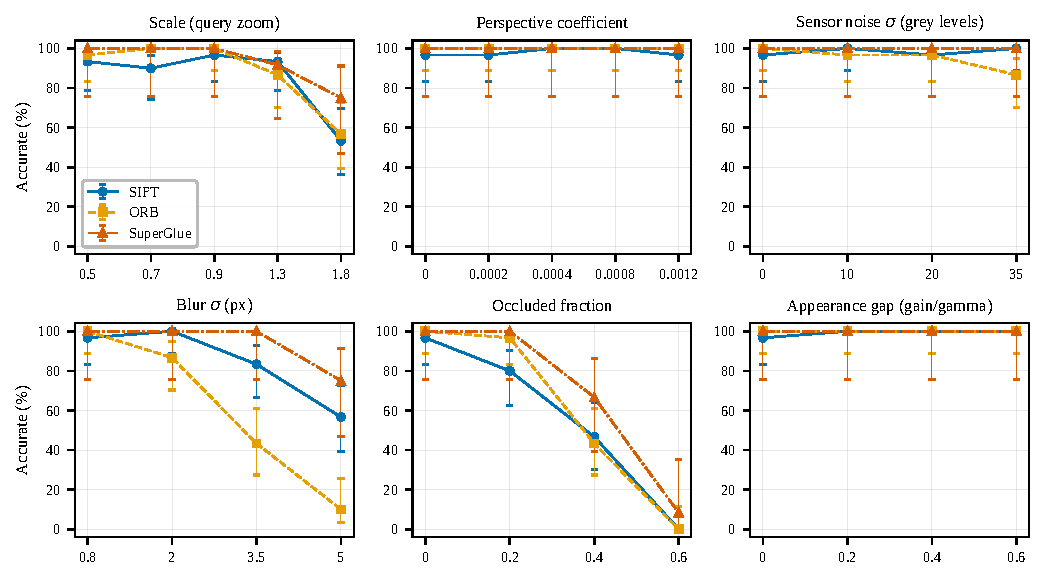
\includegraphics[width=0.98\textwidth]{figures/fig_axes_v2.pdf}
\caption{Accurate localizations against six degradation axes, with 95\% Wilson intervals (30 trials per cell for SIFT and ORB, 12 for SuperGlue). Rotation is $15^\circ$ throughout.}
\label{fig:axes}
\end{figure*}

\begin{table}[t]
\centering
\caption{Hardest tested level of each axis: accurate\,/\,silent-failure rate (\%).}
\label{tab:axes}
\begin{tabular}{@{}llccc@{}}
\toprule
Axis & Level & SIFT & ORB & SuperGlue \\
\midrule
Scale (zoom) & 1.8 & 53 / 33 & 57 / 17 & 75 / 8 \\
Perspective & 0.0012 & 97 / 3 & 100 / 0 & 100 / 0 \\
Sensor noise & 35 & 100 / 0 & 87 / 13 & 100 / 0 \\
Blur & 5 & 57 / 0 & 10 / 10 & 75 / 17 \\
Occlusion & 0.6 & 0 / 73 & 0 / 67 & 8 / 75 \\
Appearance gap & 0.6 & 100 / 0 & 100 / 0 & 100 / 0 \\
\bottomrule
\end{tabular}
\end{table}

\subsection{A confidence gate on the inlier count}
Fig.~\ref{fig:gate} and Table~\ref{tab:gate} treat the RANSAC inlier count as a confidence score. On the rotation sweep, where SuperGlue is wrong in 147 of 300 trials, the inlier count separates correct from wrong results almost perfectly (AUROC 0.999): a gate that accepts at most 1\% wrong answers still keeps 51\% of trials, which is essentially the share SuperGlue gets right, so the gate rejects the silent failures without discarding correct results. The same holds on the stress axes (SuperGlue AUROC 0.999, 93\% coverage at 1\% risk), while the classical matchers separate less cleanly (SIFT 0.968, ORB 0.992) and keep 80 to 83\%. The gate converts a silent failure into a detected one, so a navigation stack can fall back to another sensor. It does not recover the lost availability: gated SuperGlue answers only about half of the rotation sweep, whereas the rotation-hypothesis variant answers all of it.

\begin{figure*}[t]
\centering
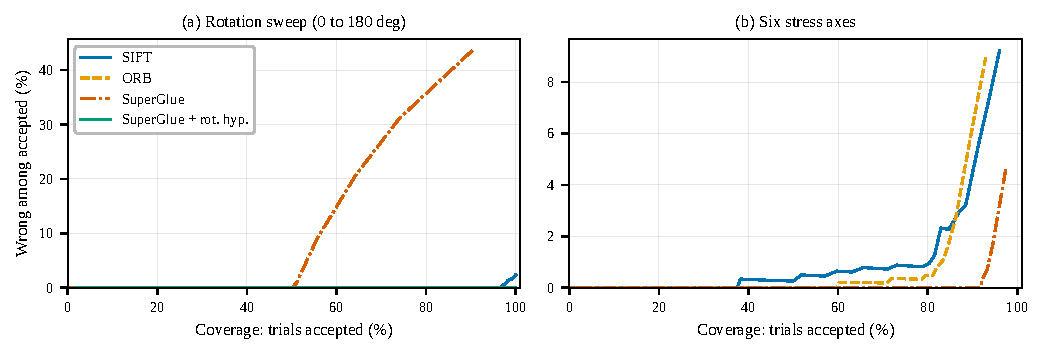
\includegraphics[width=0.98\textwidth]{figures/fig_gate_v2.pdf}
\caption{Risk-coverage curves for a gate that accepts a result when its RANSAC inlier count reaches a threshold. Lower is better; a curve that stays at zero keeps wrong answers out at every coverage. The rotation-hypothesis variant makes no wrong answers, so its curve lies on the axis.}
\label{fig:gate}
\end{figure*}

\begin{table*}[t]
\centering
\caption{Inlier-count gate. Wrong: trials that are not accurate (silent failures or no homography), as wrong/total. AUROC: probability that an accurate trial has a higher inlier count than a wrong one. Coverage: share of trials accepted at a threshold that keeps at most 1\% of accepted results wrong. n/a: no wrong trials to separate, or not run.}
\label{tab:gate}
\begin{tabular}{@{}lcccccc@{}}
\toprule
 & \multicolumn{3}{c}{Rotation sweep} & \multicolumn{3}{c}{Six stress axes} \\
\cmidrule(lr){2-4}\cmidrule(lr){5-7}
Method & Wrong & AUROC & Coverage (\%) & Wrong & AUROC & Coverage (\%) \\
\midrule
SIFT & 7/300 & 0.995 & 98 & 100/780 & 0.968 & 80 \\
ORB & 0/300 & n/a & 100 & 120/780 & 0.992 & 83 \\
SuperGlue & 147/300 & 0.999 & 51 & 22/312 & 0.999 & 93 \\
SuperGlue + rot.\ hyp. & 0/108 & n/a & 100 & n/a & n/a & n/a \\
\bottomrule
\end{tabular}
\end{table*}

\subsection{A second texture domain}
To check that the cliff is not an artifact of the procedural scenes, we repeated the rotation sweep on the photographic ground-texture mosaic (20 trials per cell for SIFT and ORB, 12 for SuperGlue, 8 for the rotation-hypothesis variant). SIFT (95 to 100\% accurate) and ORB (90 to 95\%) again stay flat over $0^\circ$ to $180^\circ$. SuperGlue is 100\% accurate at $0^\circ$ and 92\% at $30^\circ$ and $45^\circ$, then 33\% at $60^\circ$ and 0\% at $90^\circ$, $135^\circ$ and $180^\circ$, where 67 to 92\% of trials are silent failures. The rotation-hypothesis variant is accurate in all 32 trials at $45^\circ$, $60^\circ$, $90^\circ$ and $135^\circ$. The same cliff in the same angular region on a different image domain supports reading it as a property of the matcher rather than of one scene.


\section{Real-Data Check on UAV-VisLoc}
\label{sec:real}

\textbf{Setup.} We use the 40 drone frames and the satellite map of UAV-VisLoc flight 03 from the dataset's released example \cite{xu2024uavvisloc} (Fig.~\ref{fig:realdata}). The map was reduced to 4500\,px wide (about $2.3$\,m per pixel after correcting the horizontal scale for latitude, against $0.3$\,m in the original) so that it could be shared; this loses detail and hurts every matcher. A frame's true position is its recorded GPS coordinate mapped to a map pixel. Eight of the 40 frames (every fifth) served only to choose one drone resize width (280\,px) for all methods, using SIFT, and the other 32 frames are the test set. For each test frame we cut a $900\times900$ reference tile from the map around the true position at one of three random offsets (up to 250\,px, standing in for a last-known-position prior), giving 96 trials per method. The metric is the same: error of the projected frame centre, now in metres, with accurate meaning at most 25\,m, and the same three outcomes. Frame headings are not controlled: the metadata shows two flight legs whose heading field differs by about $160^\circ$.

\begin{figure*}[t]
\centering
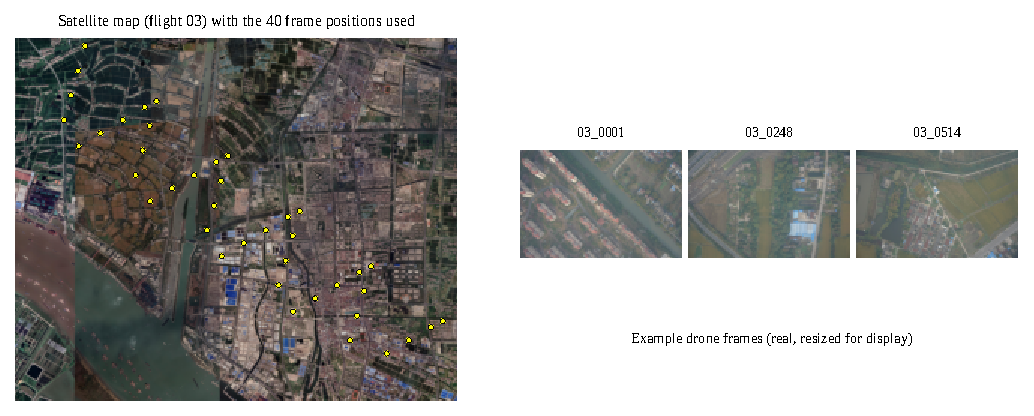
\includegraphics[width=0.92\textwidth]{figures/fig_realdata_v2.pdf}
\caption{Real data. Left: the satellite map with the 40 frame positions of flight 03. Right: three of the real drone frames.}
\label{fig:realdata}
\end{figure*}

\textbf{Results.} Table~\ref{tab:real} and Fig.~\ref{fig:realres} give the outcomes. No method is reliable on this data. SIFT is accurate in 19\% of trials (95\% CI 12 to 28) and returns no homography in 65\%. ORB is never accurate and is wrong whenever it answers. SuperGlue is accurate in 12\% (CI 7 to 21) and returns a wrong homography in 61\%, so on real data it is both less accurate and more often silently wrong than SIFT. With rotation hypotheses SuperGlue is accurate in 47\% of trials (CI 37 to 57) and almost always returns an answer, but half of those answers are wrong. Loosening the threshold to 50\,m gives 28\%, 15\% and 61\% for SIFT, SuperGlue and the rotation-hypothesis variant, with the same order.

\begin{table}[t]
\centering
\caption{Real-data outcomes at 25\,m (96 trials per method). Acc.: accurate; Silent: wrong homography; Det.: no homography. AUROC: inlier count separating accurate from other trials (undefined for ORB, which is never accurate).}
\label{tab:real}
\begin{tabular}{lcccc}
\toprule
Method & Acc. (\%) & Silent (\%) & Det. (\%) & AUROC \\
\midrule
SIFT & 19 & 17 & 65 & 0.97 \\
ORB & 0 & 28 & 72 & n/a \\
SuperGlue & 12 & 61 & 26 & 0.96 \\
SuperGlue + rot.\ hyp. & 47 & 51 & 2 & 0.91 \\
\bottomrule
\end{tabular}
\end{table}

\begin{figure*}[t]
\centering
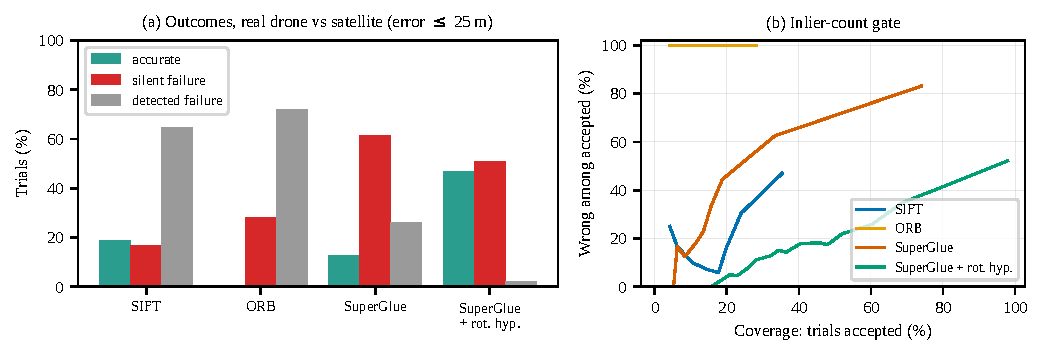
\includegraphics[width=0.96\textwidth]{figures/fig_realres_v2.pdf}
\caption{Real-data results. (a) Outcome shares per method. (b) Risk-coverage for an inlier-count gate, computed on the same trials.}
\label{fig:realres}
\end{figure*}

The rotation effect appears here too. Splitting the 96 trials by flight leg (48 each, using the heading field), SuperGlue is accurate in 12 of 48 trials on one leg and in none of 48 on the other, whose heading is about $160^\circ$ away, while the rotation-hypothesis variant is accurate in 16 and 29 of 48. Because the frames, reference tiles and matcher are identical and only the query orientation differs, the 29 successes show that those frames can be located and that SuperGlue is failing on their orientation. The two legs also cover different terrain, so the leg split alone would not prove this; the paired comparison does. No method dominates: 19 of 32 frames were located at least once, one only by SIFT and nine only by the rotation-hypothesis variant.

\textbf{Gate.} The inlier count again ranks results well (AUROC 0.91 to 0.97) but the useful range is small because correct results have few inliers on this map (median 8 for SIFT, 11 for SuperGlue, 19 for the rotation-hypothesis variant), while wrong homographies are accepted from as few as 4 inliers. For the rotation-hypothesis variant, requiring 20 inliers accepts 23\% of trials with 5\% wrong; requiring 15 accepts 34\% with 15\% wrong. These thresholds are read off the same trials and would need held-out calibration.


\section{Discussion and Limitations}
\label{sec:limits}

\textbf{Synthetic study versus real check.} In the controlled study every query is a transformed crop of its own reference, so query and reference share texture statistics, colour and local structure by construction, and the absolute accuracies will not transfer. The real check is small and has its own limits: one flight and one map (a single region and season), 32 test frames with three reference-tile offsets each, so trials are not independent and the intervals are too narrow for generalizing across frames; a reduced-resolution map; one resize width chosen on 8 frames with SIFT, which may favour SIFT slightly; ground truth that depends on the drone GPS and the map registration, whose error we did not measure; and no controlled rotation, so the heading analysis relies on a metadata field whose exact meaning we did not verify. We do not claim that the SuperGlue cliff occurs at $55^\circ$ on real imagery, only that on real frames SuperGlue fails on one heading and recovers when the query is rotated. Run times from the real runs are not reported because the jobs shared two CPU cores.

\textbf{Why the cliff.} We did not test the cause. A plausible reading is that the learned keypoint descriptors are trained largely on upright imagery and are not rotation invariant, whereas SIFT and ORB are designed to be; confirming this would need an experiment, such as retraining or augmenting with rotation, that we have not run.

\textbf{Statistical power.} SuperGlue cells on the stress axes have 12 trials, so intervals are wide, and conclusions about it relative to SIFT on those axes are suggestive. The accuracy threshold ($10$\,px, 1.25\% of the reference width) is a choice; and the gate thresholds in Table~\ref{tab:gate} are evaluated on the same trials that define the curve, so the coverage figures are optimistic and a deployed gate would need calibration on held-out data. In the synthetic study pixel error has no physical unit because the references have no ground sampling distance; the real check reports metres.

\textbf{Scope of matchers and hardware.} We evaluate one learned matcher with its public outdoor weights, which are released for non-commercial research use. LoFTR \cite{sun2021loftr} and LightGlue \cite{lindenberger2023lightglue} are not evaluated, so we make no claim about whether they share the failure. All timings are on a 2-vCPU CPU; GPU or embedded timings will differ.

\textbf{Next steps.} The full-resolution map, all 11 UAV-VisLoc flights and held-out calibration of the gate would turn this check into a benchmark. Pre-rotating the query by the recorded heading would test directly whether the rotation hypotheses can be replaced by a single pass.

\section{Conclusion}

Comparing feature matchers only by accuracy hides the property a navigation system needs most: whether a failure is noticed. On a controlled benchmark with exact ground truth, SuperGlue is the most accurate matcher in its operating range and also fails abruptly and silently outside it, returning a wrong homography in about four of five trials from $60^\circ$ of rotation upward, while SIFT and ORB degrade little. Rotation hypotheses remove the failure at four times the cost, and the RANSAC inlier count turns the silent failures into detected ones. A check on real UAV-VisLoc frames shows the same structure at much lower accuracy: every method fails often, SuperGlue is silently wrong in 61\% of trials, and rotation hypotheses raise it from 12\% to 47\% accurate. The real check is small, one flight and 32 frames, and a larger, full-resolution evaluation is the work that follows.

\bibliographystyle{IEEEtran}
\bibliography{references}

\end{document}
